\documentclass[12pt,a4paper]{article}
\usepackage[utf8]{inputenc}
\usepackage{amsmath}
\usepackage{amsfonts}
\usepackage{amssymb}
\usepackage{makeidx}
\usepackage{graphicx}
\usepackage{gensymb}

\usepackage[left=2cm,right=2cm,top=2cm,bottom=2cm]{geometry}
%\usepackage{cite}
\usepackage{xcolor}


\title{\large\textbf{Summary of the work for Week 26 \\
 from 11-01-2020 to 17-01-2020 }  }
\author{\small Gayan Lankeshwara}
\date{\small \today}

\setlength\parindent{0pt} %% changing the style to have no indentation

\begin{document}

\maketitle

During this week, my attention was focussed on the following factors.
\begin{itemize}
    \item Verifying the accuracy of the temperature model used in the study.
    \item Fine tuning the optimisation problem which was developed to chose a set of appliance within a specific cluster.
    \item Learning about GridLAB-D which could be useful tool to run and simulate DR problems in the residential network.
\end{itemize}

To sum up, fig.\ref{fig:flow_chart} is a flow diagram of the approach that I will be developing to acquire the desired capacity during a DR event.\\

\begin{figure}[htb!]
    \centering
    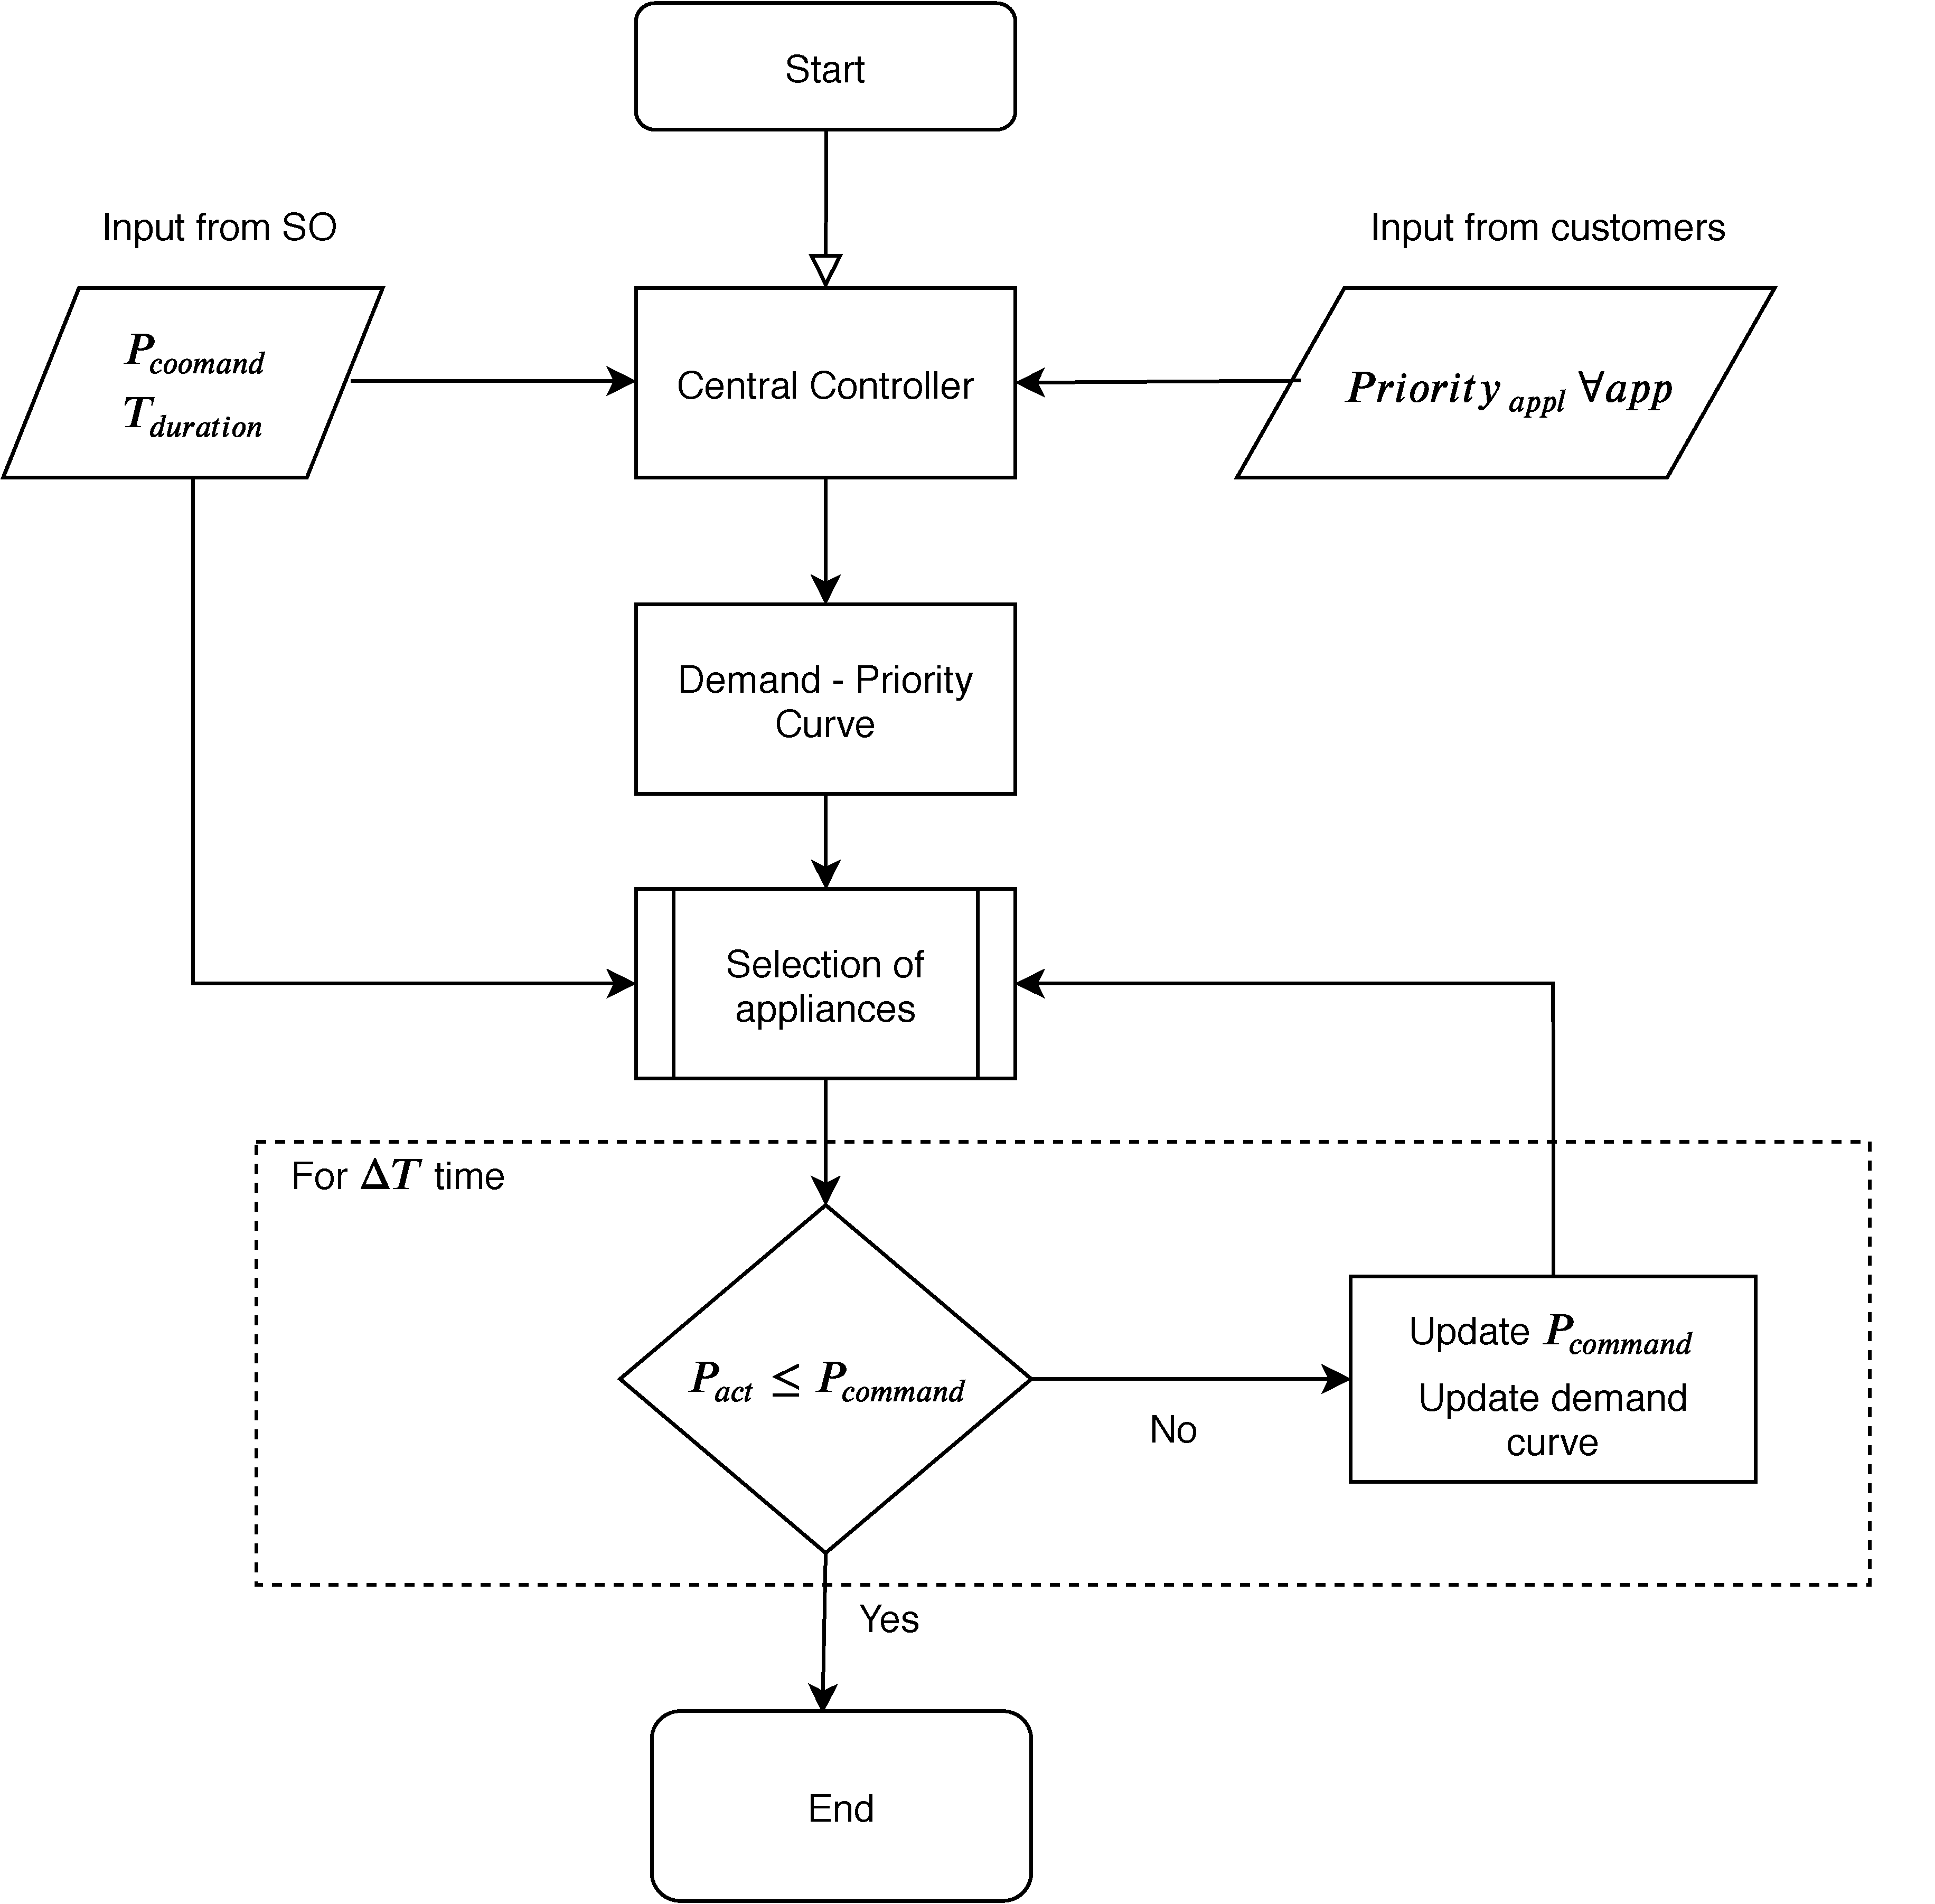
\includegraphics[width =13cm]{images/flow_chart.pdf}
    \caption{The flow chart of the proposed scheme}
    \label{fig:flow_chart}
\end{figure}

According to fig.\ref{fig:flow_chart}, the customers provide the desired priorities for appliances in a house starting from 1 (lowest) to $N$ (highest). Here N is the number of controllable appliances in a particular house. \\

In the next step, based on the priorities assigned for each appliance, the central controller cluster the appliances based on the defined priority levels. This will automatically formulate the demand-priority curve which is used for the appliance selection process.\\

During peak demand hours where the supply and demand balance can not be satisfied with the existing generation, the system operator (SO) informs the central controller that it requires a demand response of $P_{command}$ within $T_{duration}$ interval.\\ 

Here $T_{duration}$ can be minutes or hours depending on the requirement. For example, if the action is a peak-shaving it will in hours but if it is bidding in markets or ancillary services, it will be in minutes. \\

In the next step, the central controller goes through the demand priority chart to chose the appliances which are going to participate in the demand response. Once it selects a certain cluster of appliances, an optimisation process will be run only within that cluster to determine the set of appliances that should be controlled.\\


Following are the assumptions made in the process.
\begin{itemize}
    \item \textcolor{red}{Central controller is able to see the states and corresponding power levels of each appliance in a particular house. It is believed that the existing infrastructure can provide access to those details either through sensors connected or else with load disaggregation techniques.} 
    \item Customers are able to override any DR event if they are not satisfied with the comfort violation or else due to personal reasons. \textcolor{red}{But it is absolutely required to define an upper margin for the number of attempts in which the event can be overridden, in order to have a guarantee that the DR can be achieved.} 
\end{itemize}

The selection process is done by the central controller based on the demand-priority chart developed at a particular time step $t$. In order to select the appliances within a certain cluster of, an optimisation process will be conducted.\\

Considering a \emph{step-ahead optimisation approach},

\begin{equation}
    F =\, min \sum_{i=1}^{N_{tot}}\, [\,\alpha \, C_{i}\cdot P_{i} + \beta\, CI_{i}^2\,] \quad \quad \forall \: i
\end{equation}
\\

\textbf{Decision variables : $P_{i}$ and $T_{i,t}^{room}$}\\

$\alpha$ and $\beta$ are weighting parameters \\

In order to properly define the weighting parameters $\alpha$ and $\beta$, normalisation of the objective functions has to be done \cite{Marler2010}.
\begin{equation}
    F_{i} = \frac{f_{i}- f_{i,min}}{f_{i,max}-f_{i,min}} \quad \quad  \forall \:i
\end{equation}

where \\

$f_{i,min}$ is the objective value when $f_{i}$ was minimised independently (\emph{Utopia point}). \\

$f_{i,max}$ is the maximum value of $f_{i}$ when the other objectives are minimised, which is\\  
$max_{1\leq j \leq k } f_{i}(x^{(j)})$ (\emph{nadir point})

\subsection*{\small Constraints}
\begin{align}
    \label{eq: power_balance}
    \sum\limits_{i} P_{i,t} &= P_{i,t}^{demand} \quad \forall t \\
     \label{eq: CI_intro}
    CI_{i,t} &= \frac{2T_{i,t}^{room}- T_{i}^{low}-T_{i}^{high}}{T_{i}^{high}-T_{i}^{low}} \quad \quad \forall \: i,t\\
     \label{eq: Temp_limits}
    T_{i}^{low} &\leq T_{i,t}^{room} \leq  T_{i}^{upper}\quad \quad \forall \: i,t \\
    \label{eq: Power_limits}
    P_{i}^{min} &\leq P_{i,t} \leq  P_{i}^{max}  \quad \quad \forall \: i,t \\
     \label{eq: Indoor_temp_model}
    T_{i,t}^{room} &= T_{i,t}^{out} - Q_{i,t}\cdot R_{i} - (T_{i,t}^{out} - Q_{i,t}\cdot R_{i}
    - T_{i,t-1}^{room})\cdot e^{-\frac{\Delta T}{R_{i}C_{i}}}  \quad \quad \forall \: i,t\\
    \label{eq: Inverter_AC_model}
    Q_{i,t} &= \frac{c_{i}}{a_{i}}\cdot P_{i,t} + \frac{a_{i}\, c_{i}- b_{i}\, d_{i}}{a_{i}} \quad \quad \forall \: i,t \\
    \label{eq: power_levels_for_apps}
    P_{i,t} &= \{0.50\cdot P{i}^{rated}, 0.75\cdot P{i}^{rated}, P{i}^{rated} \}
  \end{align}
  
  
\subsection*{\normalsize A review of the Temperature model considered in the study}

\begin{itemize}
    \item Temperature model for an inverter type air conditioner was considered.
    
    \item The relationship between the cooling power (Q) and the electrical power (P) with the compressor frequency (f) can be expressed as in \cite{7890446}
    \begin{align}
        \label{equation:1}
        Q &= a\cdot f + b \\
        \label{equation:2}
        P &= c\cdot f + d
    \end{align}
  
  where,\\

$a$, $b$, $c$ and $d$ are parameters which depends on the type and internal parameters of the air conditioner.\\

By combining \ref{equation:1} and \ref{equation:2}, the relationship between $P$ and $Q$ can be obtained which is,

\begin{equation}
    \label{eqn: P_and_Q}
    Q = \frac{a}{c}\cdot P + \frac{b\,c -a\,d}{c}
\end{equation} \\ 


From the first order equivalent thermal parameter model ($ETP$) as in \cite{6168821},
\begin{equation}
    \label{eqn: thermal_model}
    C\cdot \frac{dT_{in}}{dt} = \frac{T_{out}-T_{in}}{R} -\,Q
\end{equation}

where,\\

$C$ is the thermal capacity\\
$R$ is the equivalent thermal resistance\\
$T_{in}$ is the indoor temperature\\
$T_{out}$ is the outdoor temperature\\


Equation \eqref{eqn: thermal_model} can be illustrated as a difference equation which is given by \cite{8750809},
\begin{equation}
    \label{eq:discretised_ETP_model}
    T_{t+1}^{in} =  T_{t}^{out} - Q\cdot R - (T_{t}^{out}-T_{t}^{in}-Q\,R)\,e^{\frac{-\Delta T}{R\,C}} %% coreect the equation
\end{equation}

Equations \eqref{eqn: P_and_Q} and \eqref{eq:discretised_ETP_model} were combined together to get the temperature update for different electrical power values of the inverter air conditioner.\\

Simulations were performed considering several scenarios.

The values of parameters used in the simulations are \cite{7890446},
%% addd the set of parameters considered in the study
\begin{verbatim}
    a = 0.060 
    b = -0.300 
    c = 0.030 
    d = -0.40 
    R = 2 
    C = 2
\end{verbatim}



\textbf{Assuming a time step of $\Delta T$ = 15 mins}

\begin{enumerate}
    \item $T_{out}$ = 34$\degree$ and the initial room temperature is 24$\degree$. In the next step, the air conditioner is switched off due to a demand response event. ($P=0$) 
    
    \item $T_{out}$ = 34$\degree$ and the initial room temperature is 24$\degree$. In the next step, the air conditioner is undergoes different levels of power reduction due to demand response.
    
    \item $T_{out}$ = 34$\degree$ and the initial room temperature is 24$\degree$. In the next step, the air conditioner is undergoes a constant power reduction to keep the room temperature remains at the initial value.
    
\end{enumerate}

\subsection*{Considering situation 1,}

\begin{figure}[htb]
    \centering
    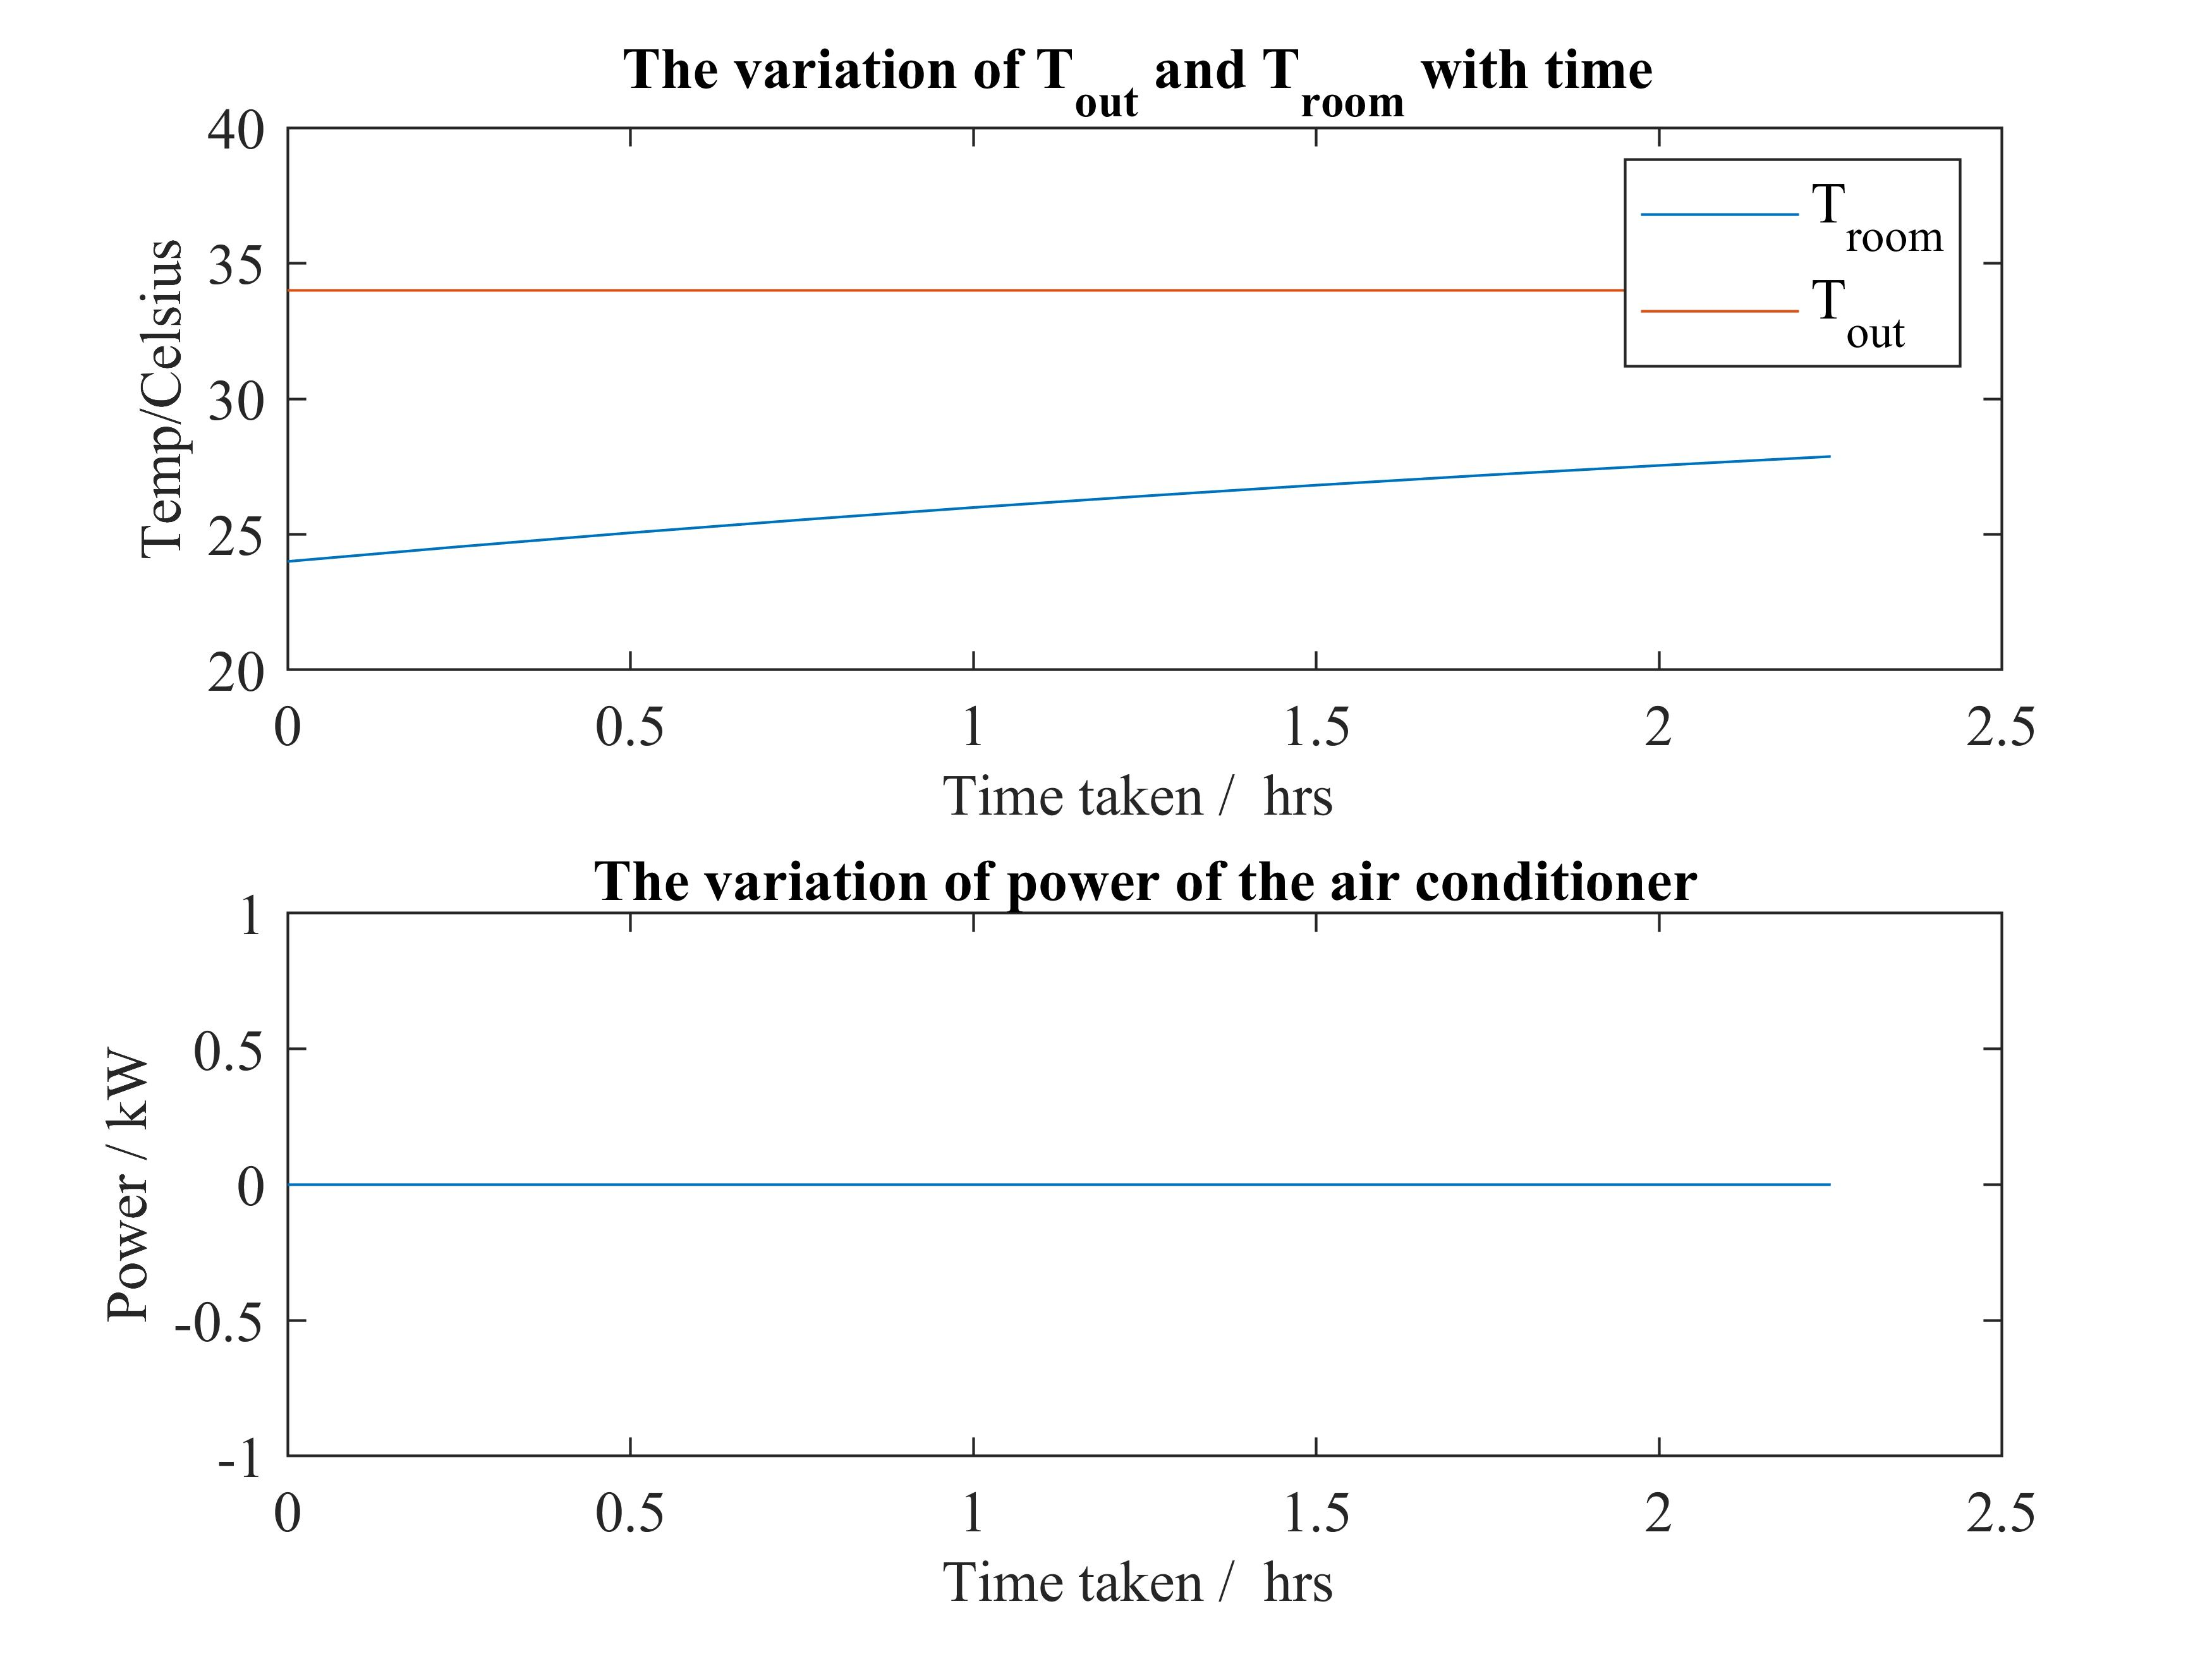
\includegraphics[width=13cm]{images/power_at_zero.jpg}
    \caption{The variation of room temperature with time}
    \label{fig:zeropower}
\end{figure}

According to figure \ref{fig:zeropower}, it is obvious that it takes a very long time for indoor temperature to reach the outdoor temperature when the air conditioner is switched off.\\

It is further elaborated with the following figure,

\pagebreak
\begin{figure}[htb]
    \centering
    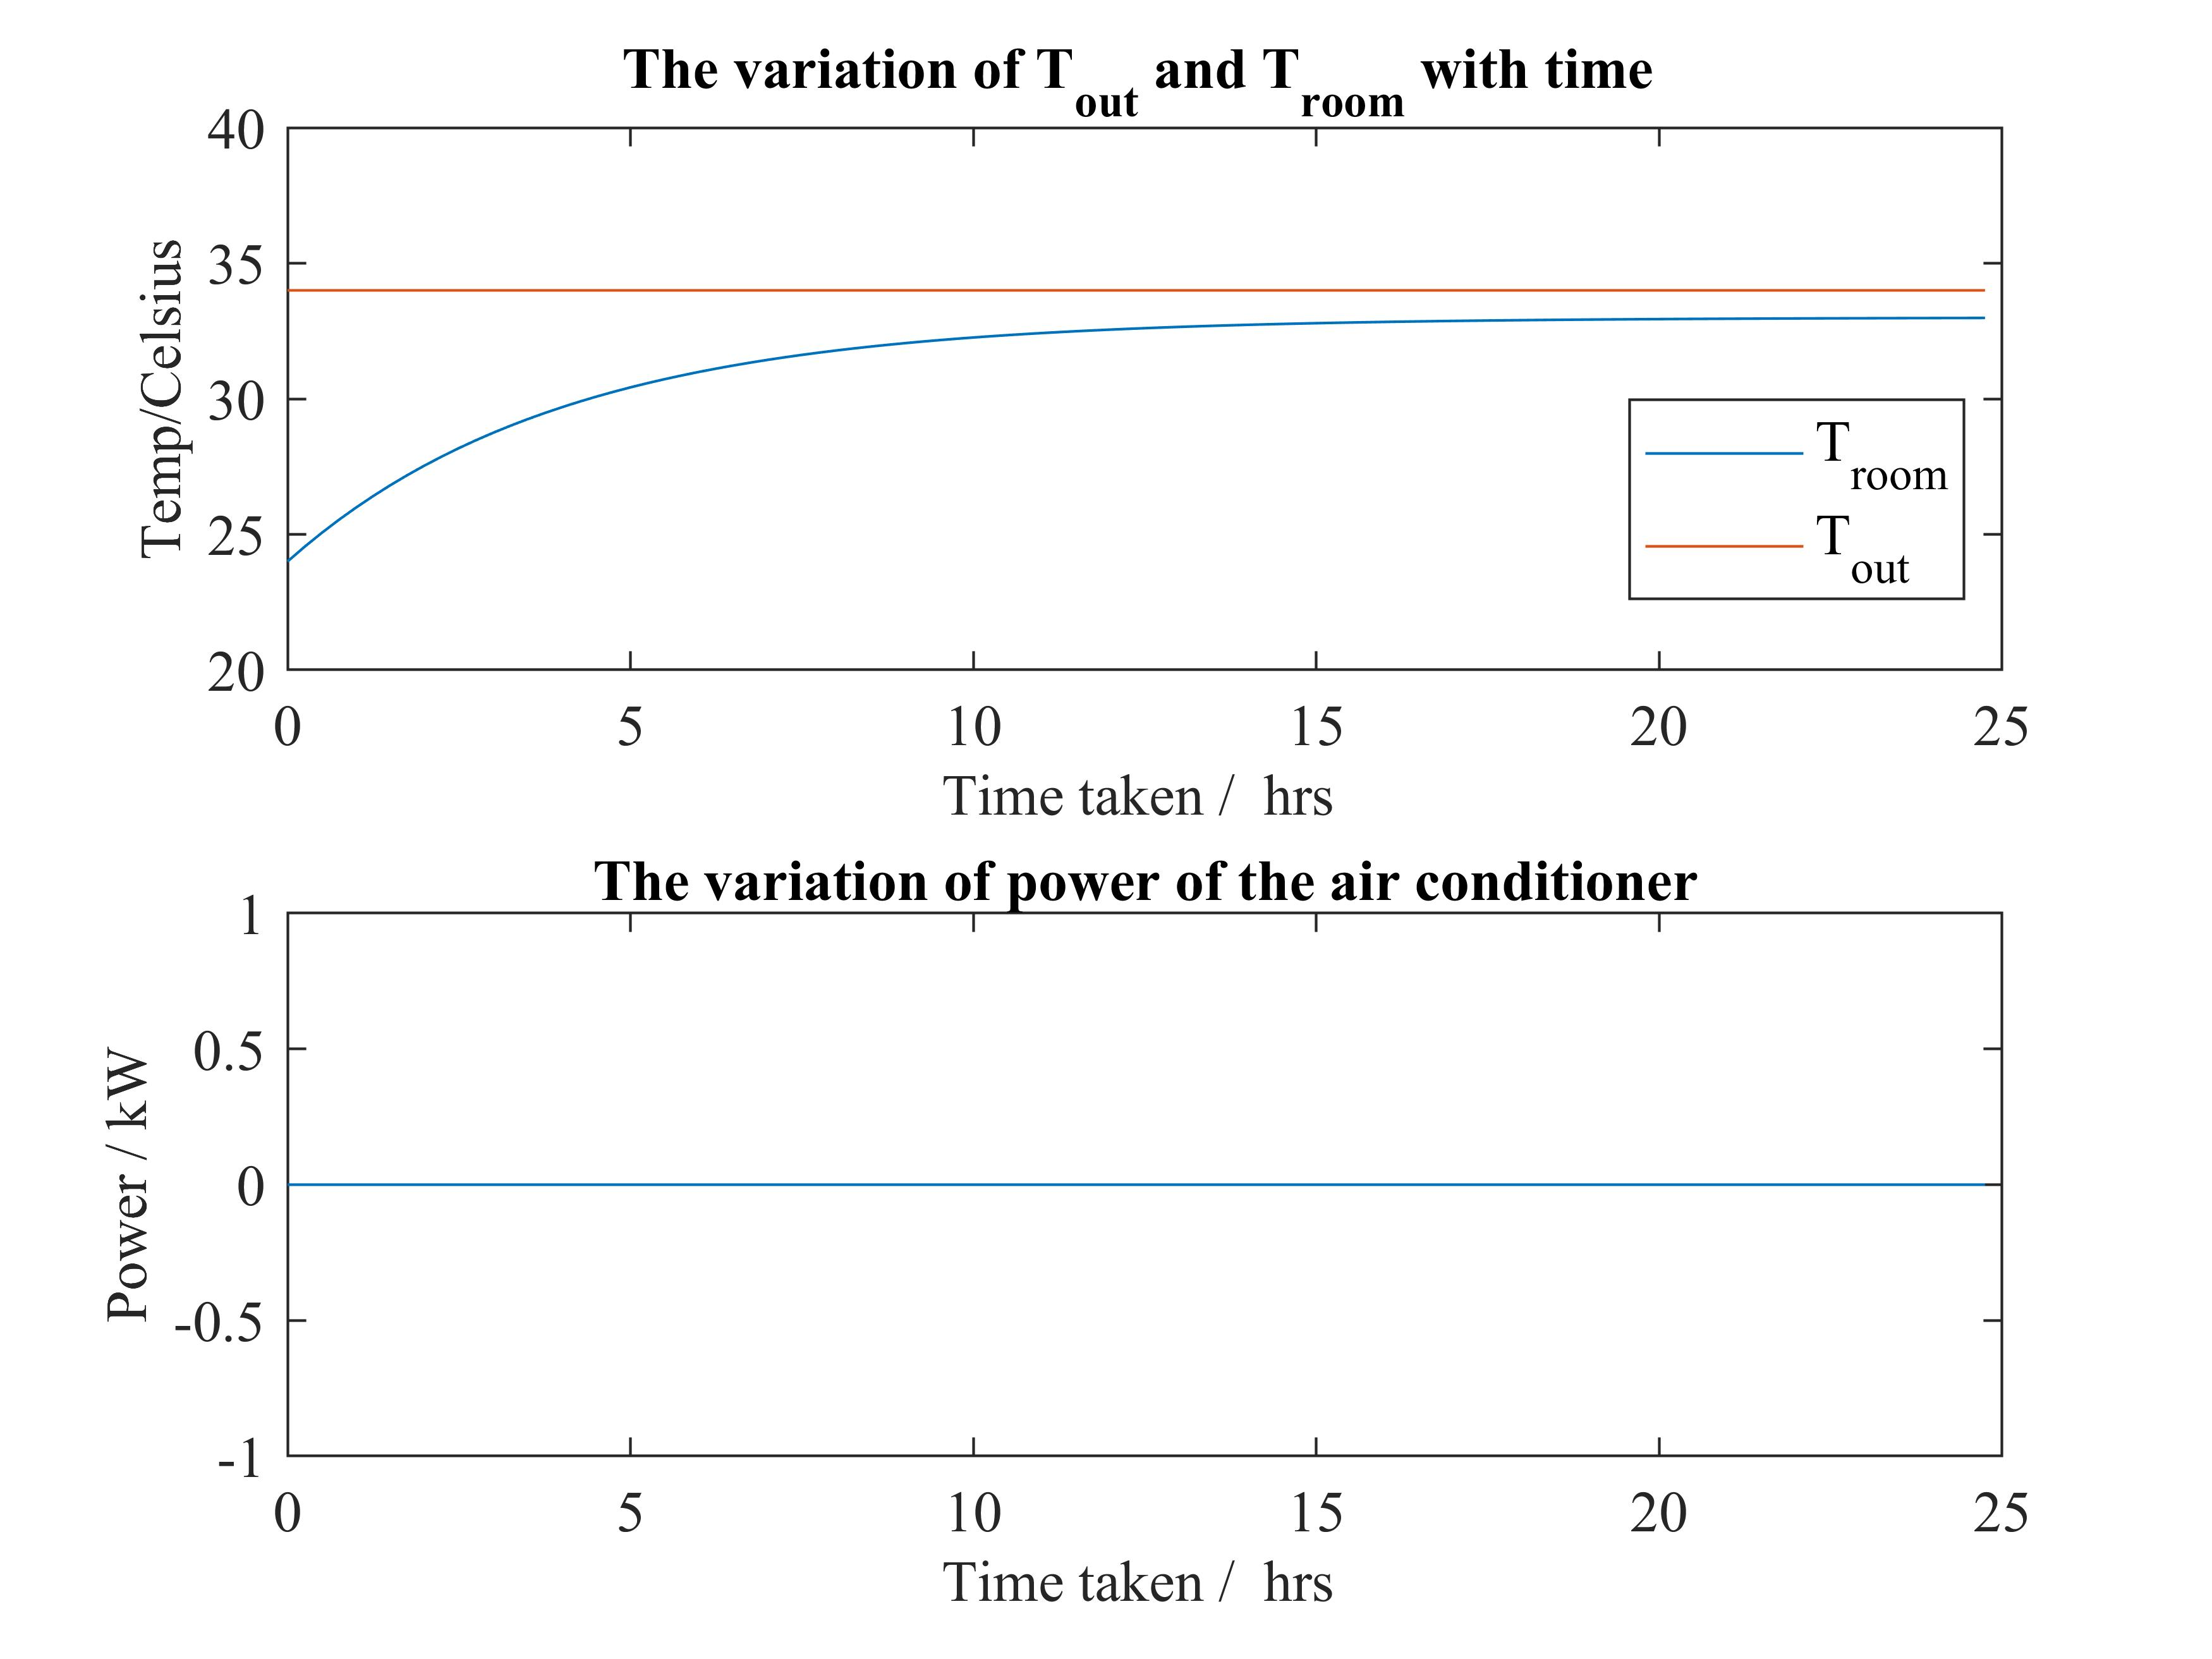
\includegraphics[width=13cm]{images/power_at_zero_long_iterations.jpg}
    \caption{The variation of room temperature with time for a longer period of time}
    \label{fig:zeropower_with_log_iterations}
\end{figure}
\end{itemize}


\subsection*{Considering situation 2,}

Electrical power output of the air conditioner was varied in different discrete levels to observe the how it affects the indoor temperature.

\begin{figure}[h!]
    \centering
    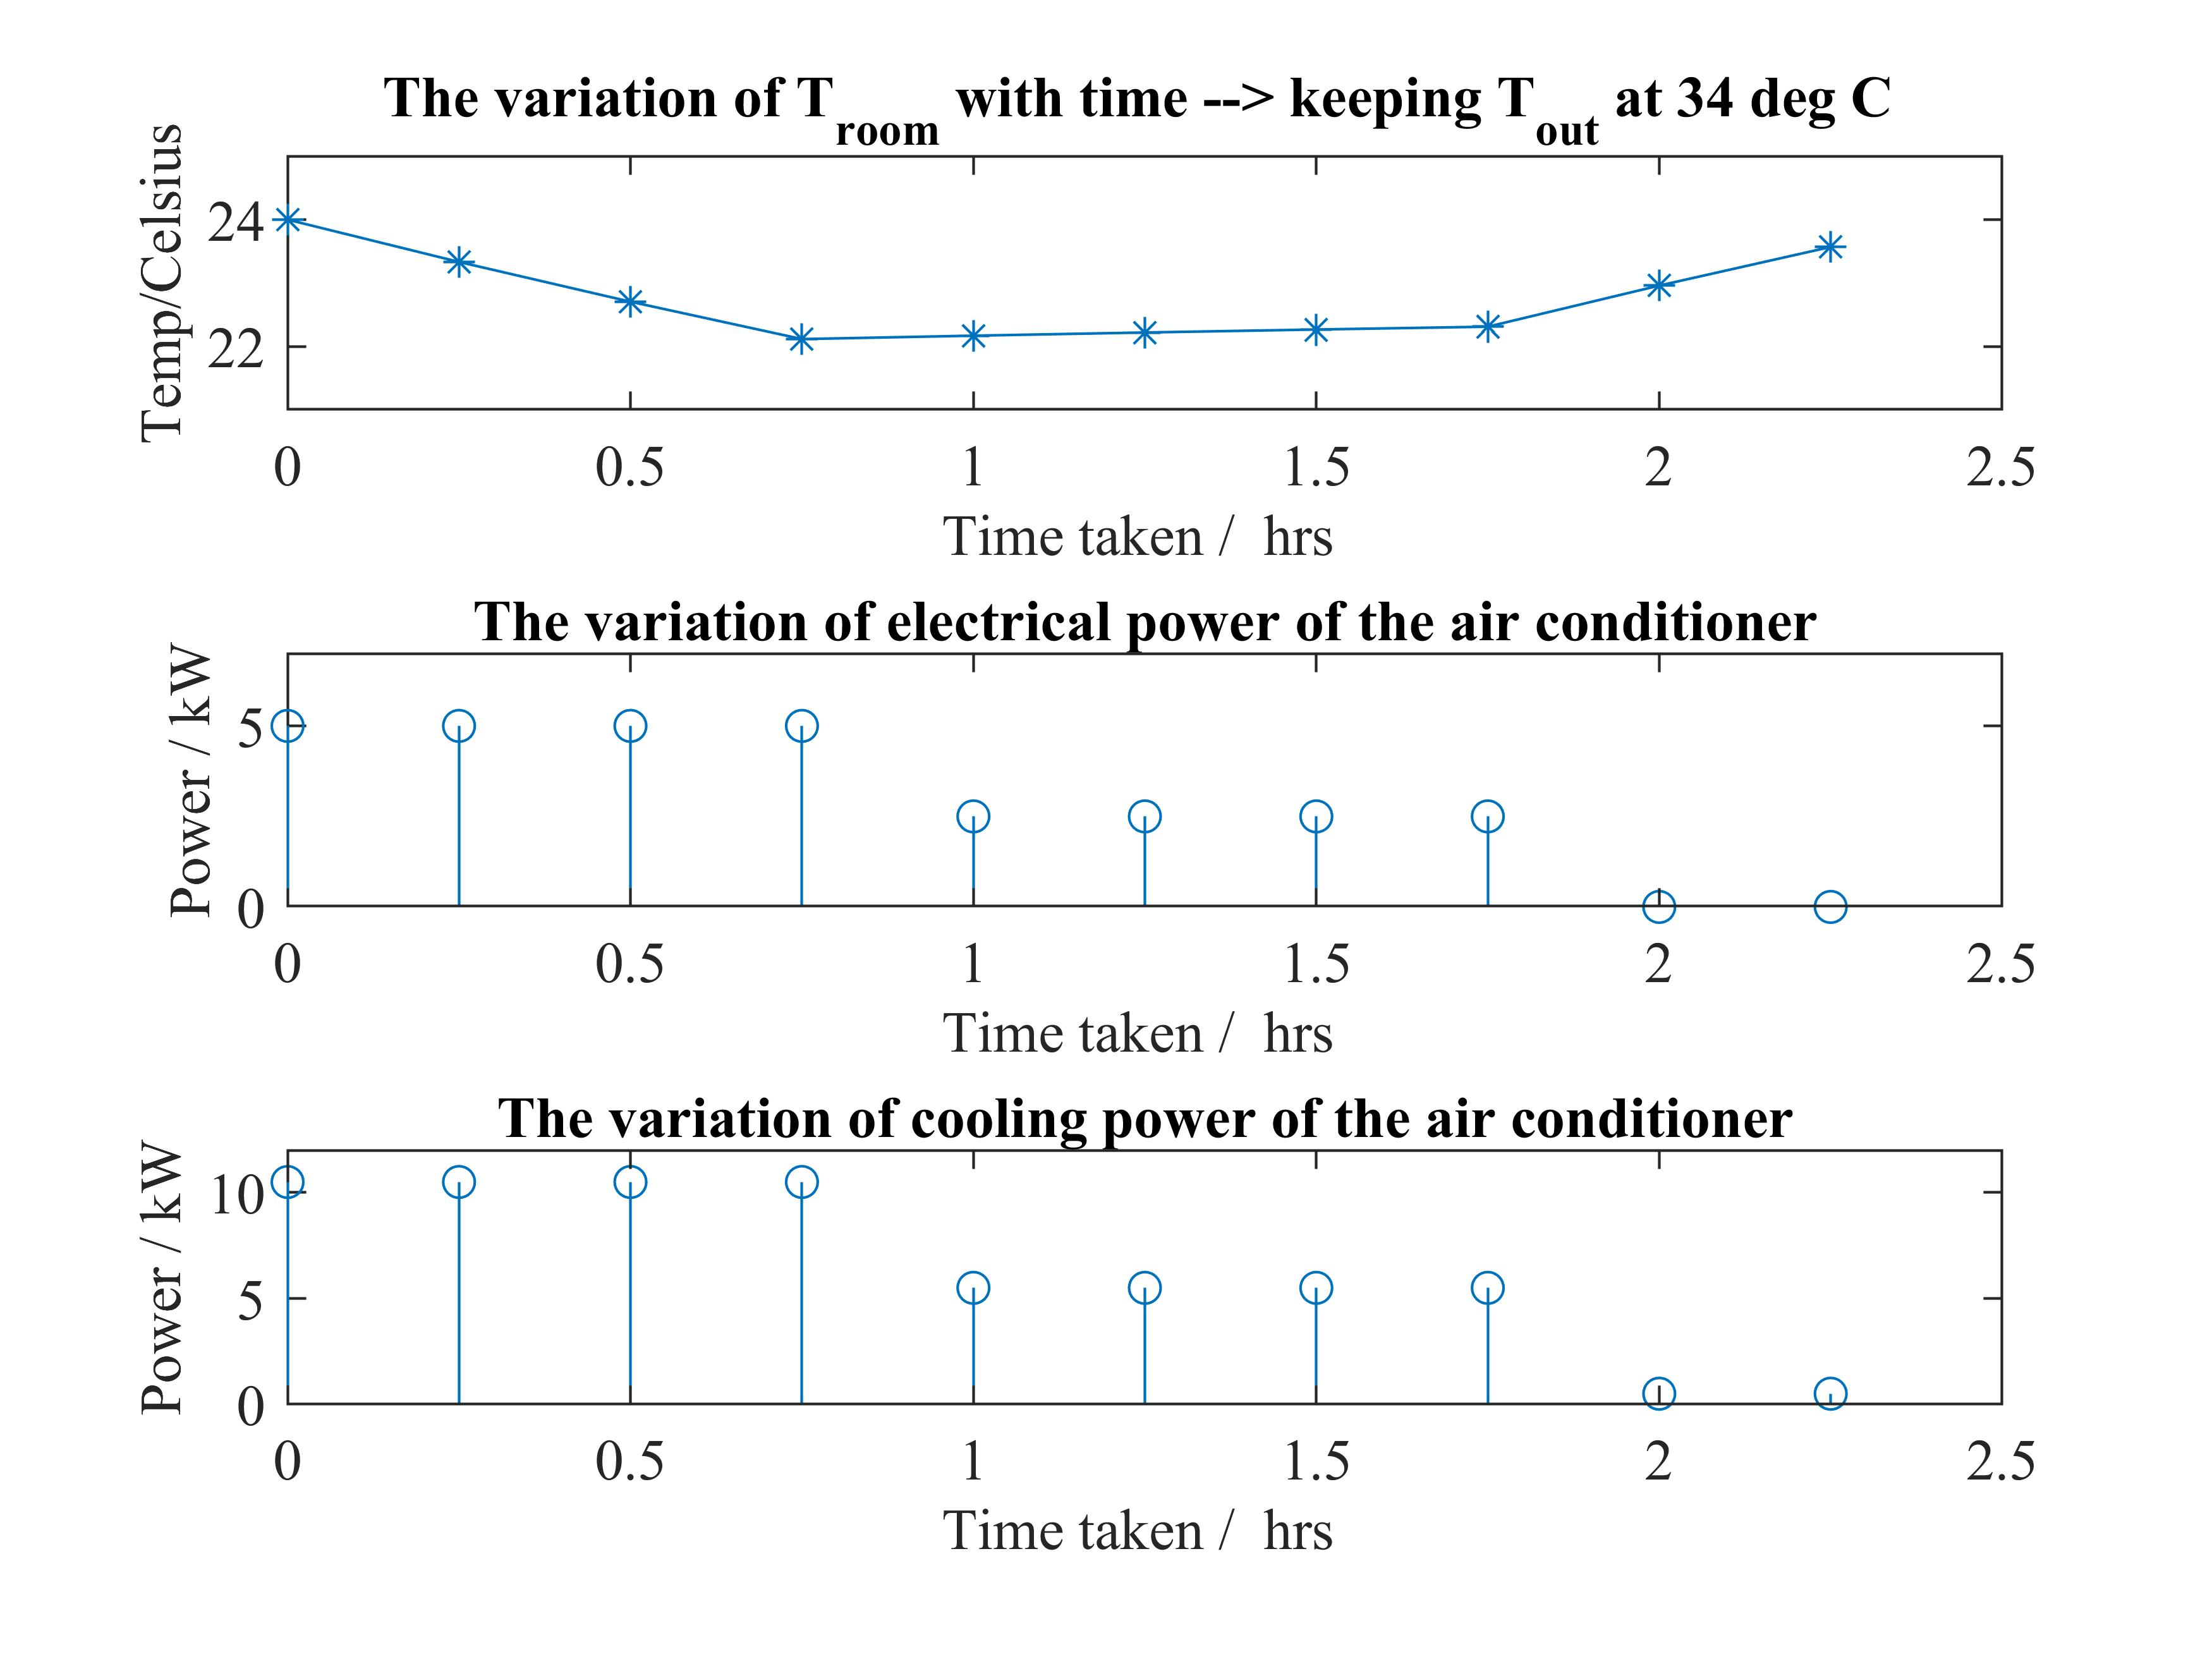
\includegraphics[width=13cm]{images/for_varying_power_levels_with_Q.jpg}
    \caption{The variation of indoor temperature for different power levels of the air conditioner}
    \label{fig:my_label}
\end{figure}

The initial temperature was 24\degree C. Until 45 mins, the air conditioner operated at the rated power of 5 kW. So the temperature dropped. Thereafter the air conditioner kept operating at 2.5 kW (half power) for 1 hour where the temperature slowly increased. Finally the air conditioner was switched off during which the temperature increased rapidly.\\

Another important point to consider here is that although P was zero for the last two time steps, the cooling power was not exactly zero.\\


\subsection*{Considering situation 3,}

In scenario 3, it was required to identify the cooling power as well the electrical power that should be supplied to keep the indoor temperature operating at 24\degree C while the outdoor temperature remains at 34\degree C.\\

With equation \eqref{eq:discretised_ETP_model},

\begin{equation}
    T_{t+1}^{in} = T_{t}^{in} = T_{t}^{out} - Q\cdot R
\end{equation}

\begin{figure}[h!]
    \centering
    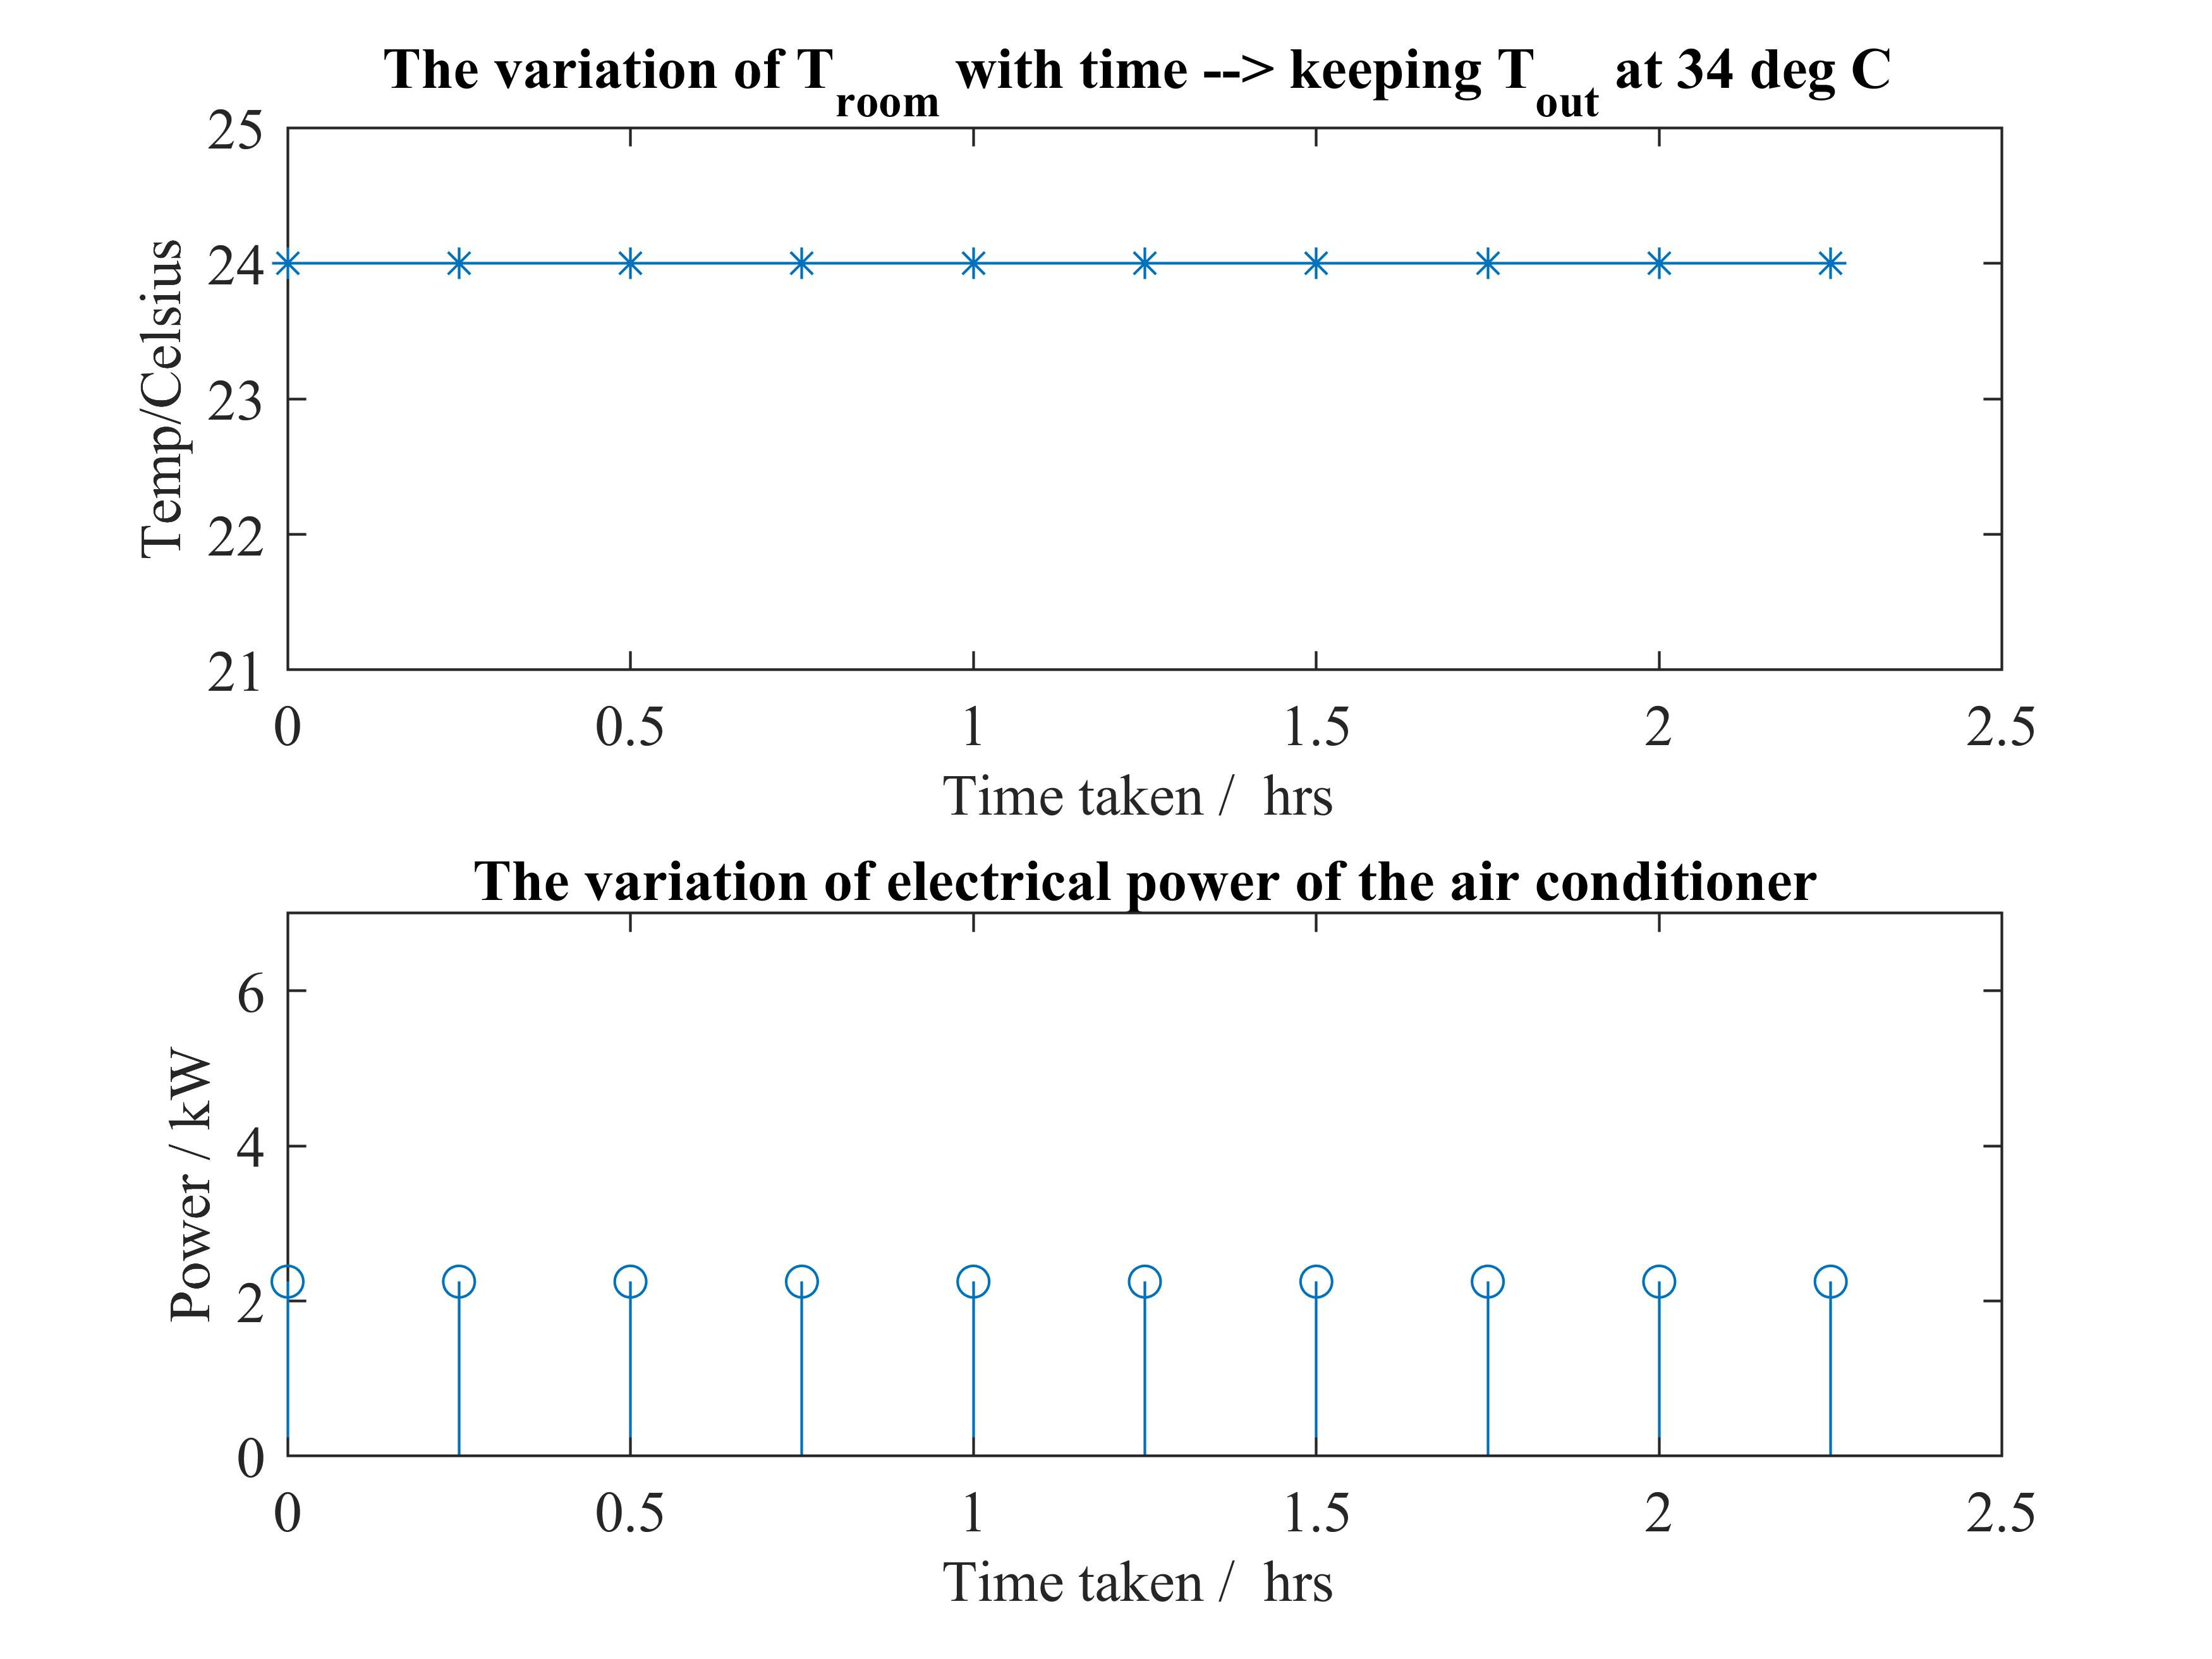
\includegraphics[width=13cm]{images/constant_P_and_T.jpg}
    \caption{The variation of indoor temperature with electrical power}
    \label{fig:constant_P}
\end{figure}

As long as the cooling power Q = 5 kW and P = 2.25 kW, the indoor temperature which was initially at 24\degree C remains constant.

\subsection*{Considering situation 4,}

The lower limit and the upper limit of the set point temperature was assumed to be 22\degree C and 27\degree C respectively. Thereafter the behaviour of the room temperature within the predefined limits were studied for the case where the demand response occured when the room temperature was 24\degree C.

\pagebreak

\begin{figure}[htb!]
    \centering
    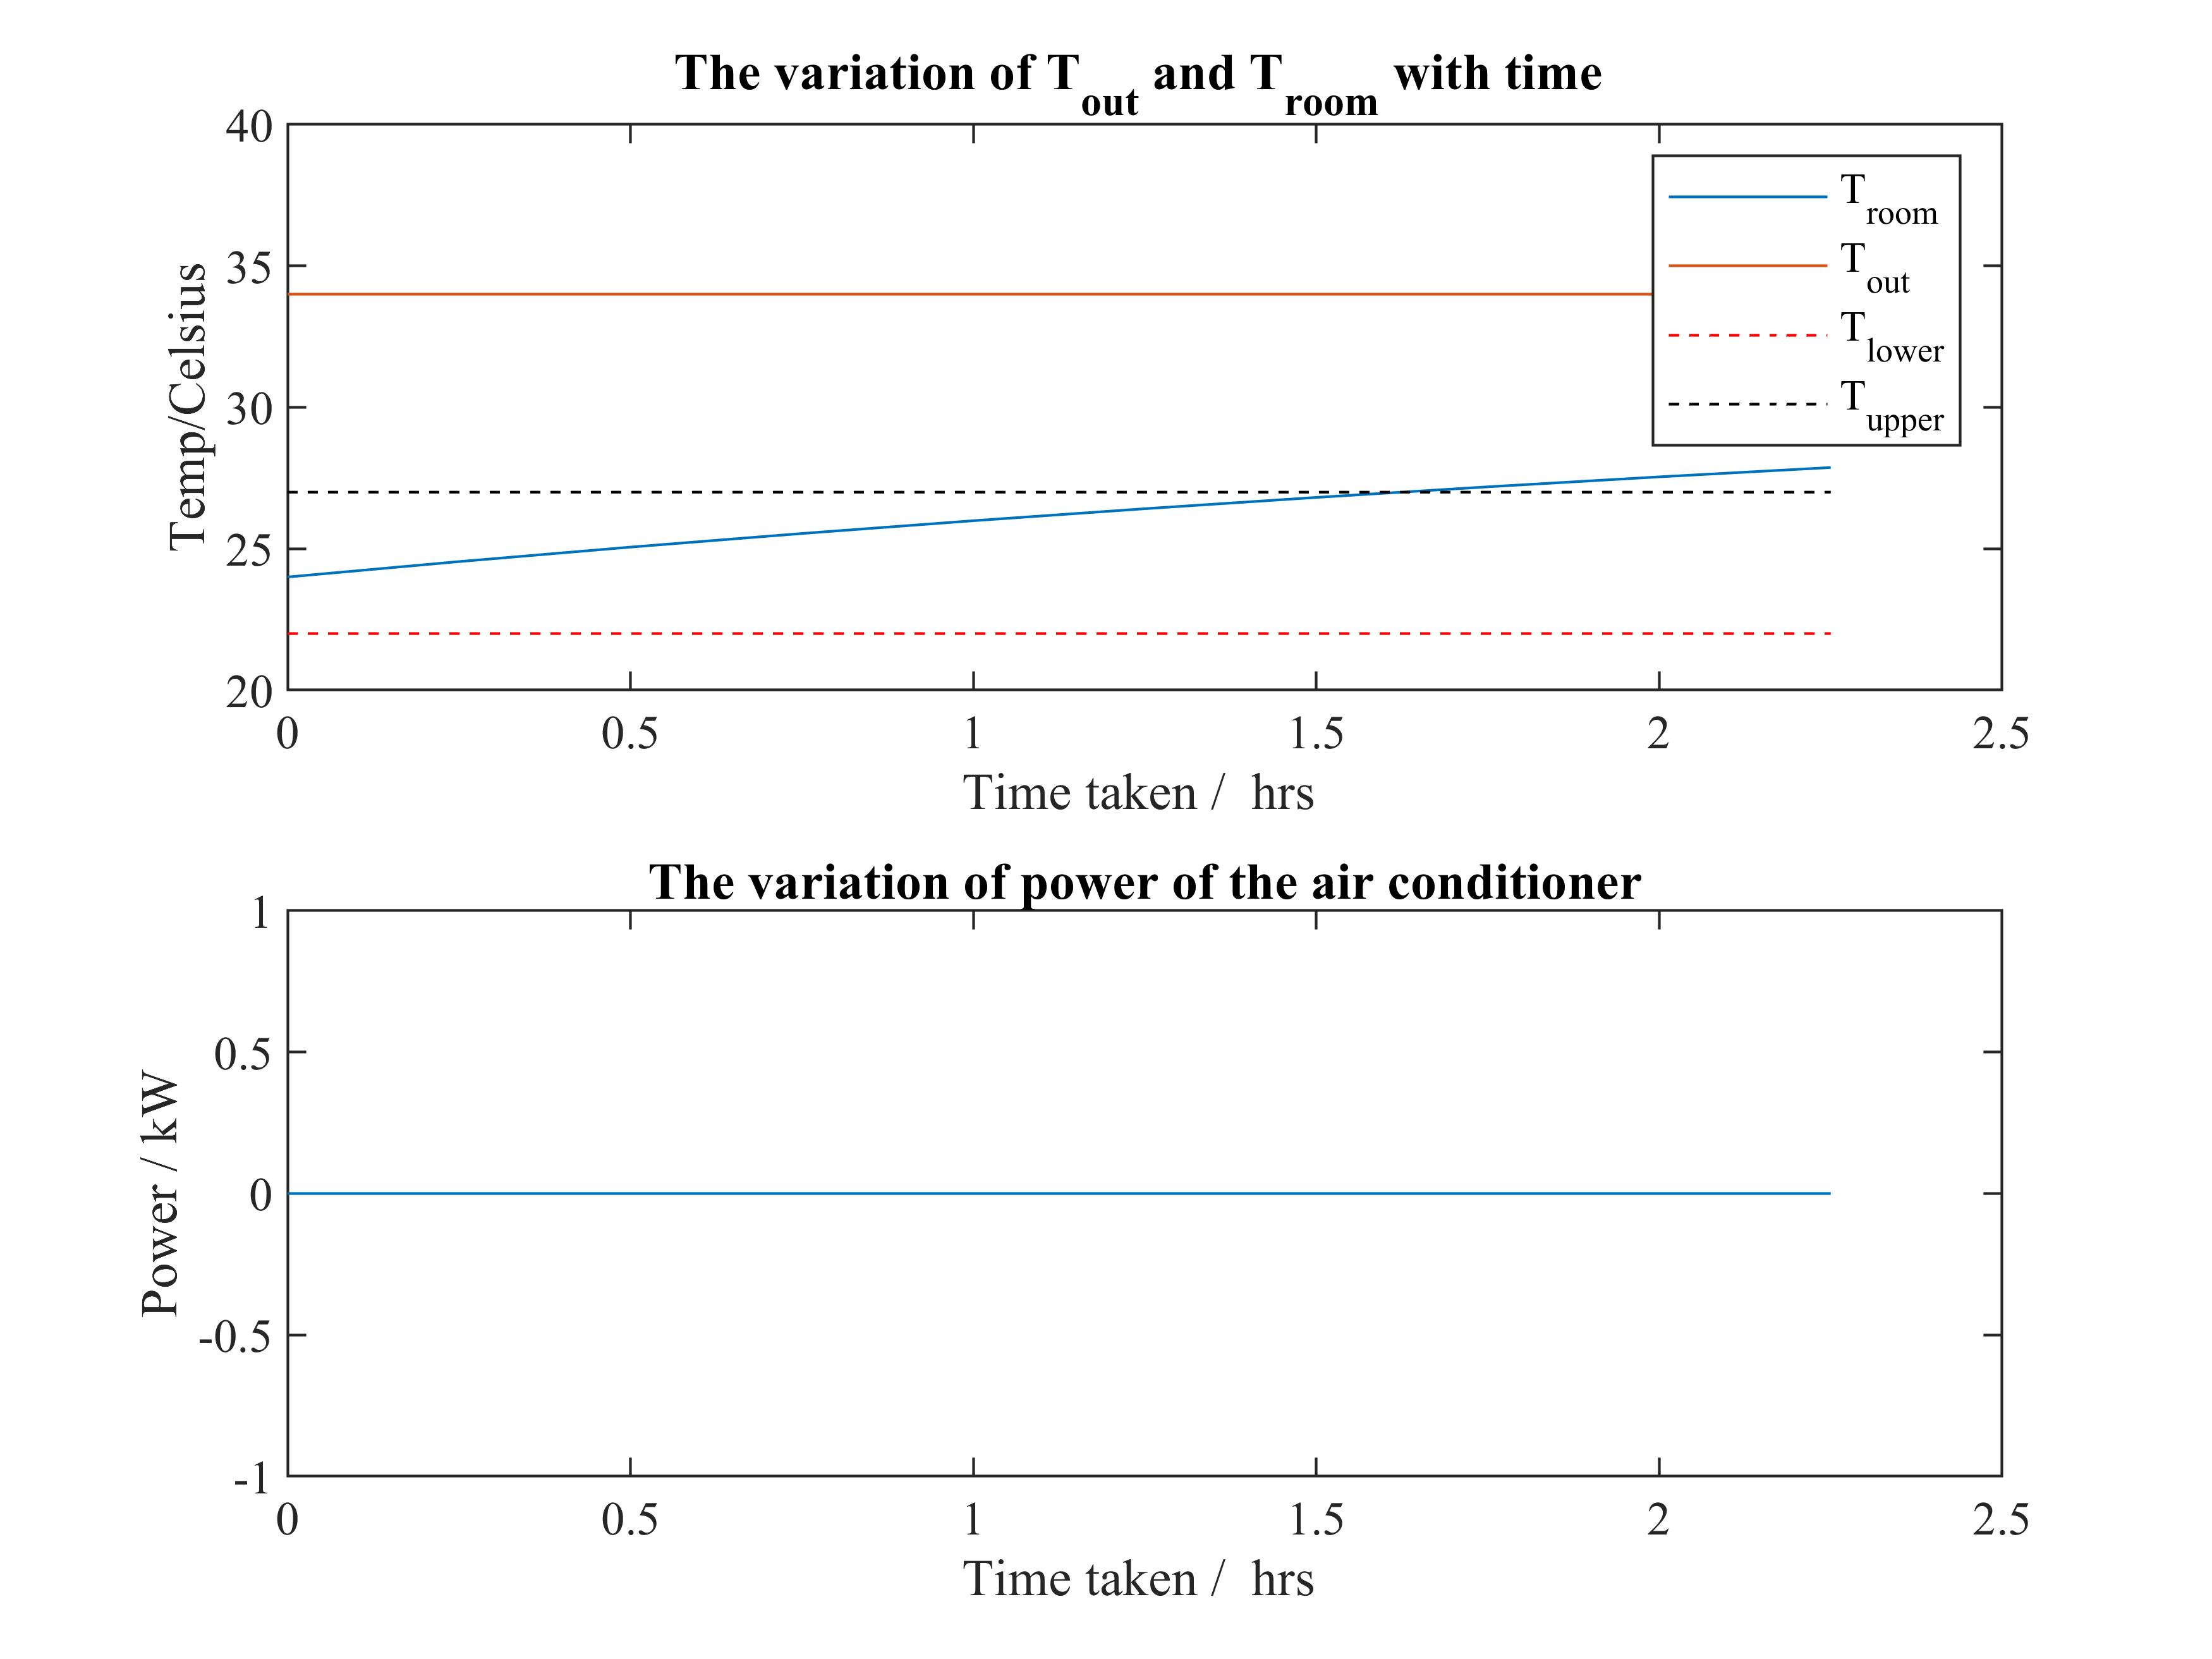
\includegraphics[width=14cm]{images/power_at_zero_with_set_limits.jpg}
    \caption{Variation of room temperature during the demand response event}
    \label{fig:with_set_limits}
\end{figure}

\textcolor{red}{From figure \ref{fig:with_set_limits} it was observed that the room temperature violates the upper level of the set point temperature only after 1.5 hrs once the air conditioner is completely switched off.} \\

\textcolor{red}{Hence there arises the question "Why do we need to control the power at discrete levels instead of switching off the device completely during the demand response event because switching off the device will not cause harm at all until 1.5 hrs from the beginning of the event."}




\subsection*{Some of the ideas that need to be considered in future work}

\begin{itemize}

\item How am I going to incorporate the \emph{overriding capability }in my algorithm ?

\item Deciding the range for $T_{duration}$ provided by the system operator is essential. Because the action of load control that we achieve significantly depend on this parameter. Not only that $T_{duration}$ will decide type of the problem that we are going to tackle with.\\

For example, \\

if $T_{duration}$ is in $hours$  peak shaving problem.\\
if $T_{duration}$ is in $minutes$ $\longrightarrow$ market clearing problem, ancillary services.\\

But if we consider the problem in our hand, I think we need to deal with \textcolor{red}{emergency demand response (EDRP)} \cite{7063260,SIANO2014461,6861959} problem.

    \item Currently we are only focussing on air conditioning loads for the DR. If we are going to incorporate the task based appliances such as dish washers, washing machines and cloth dryers, there arises a question how are we going to control them. For the air conditioners, controlling can be achieved by reducing the power consumption but for time-shiftable loads, such kind of a approach is not valid. 
    
    \item Modelling the discomfort for the time shiftable appliances need to be considered for the optimisation problem.
    
    \item Need to think about the price parameter for the aggregator cost. Two approaches are possible over here. One is modelling the cost as a conventional quadratic cost function such as $C(P_{i})= a\cdot P_{i}^2+b\cdot P_{i}+c$. If so we need to determine the parameters for a,b and c. If not we can assume that \emph{spot price of electricity} is available as an input and it can be used directly. Simply,\\
    
\textbf{Are time shiftable loads capable of providing emergency demand response ???}\\
    
    \item The temperature model considered in the study seems not to be that much effective because the temperature drop once an air conditioner is fully controlled is still not that significant to the case where it is not controlled and operating at the rated power. The accuracy of the model heavily depends on the parameters that we considered for a,b,c,d, R and Ca. Hence much attention needs to be paid over there.
    
    \item Another issue with the developed algorithm is deciding for long the appliances are operating under the controlled mode once demand response is enabled over there. Because as long as the appliance is operating under the controlled state, the room temperature tends to increase most of the time and at one point, the temperature will violate the limits assigned by the user, which is not acceptable.
    
    \item If we are controlling the appliances in a lower cluster, do we need to look for the comfort index of those appliances as well. This can be justified with the fact that if a user assigns a lower priority for an appliance, it does mean that he will not that much bother if that appliance was controlled at a certain time step.
\end{itemize}


\bibliographystyle{ieeetr}
\bibliography{referenceList}


\end{document}